\documentclass[uplatex, a4paper, 12pt, openany, oneside]{jsbook}

\usepackage[dvipdfmx]{graphicx}
\usepackage[dvipdfmx]{color}
\usepackage[dvipdfmx, bookmarks=true, setpagesize=false, hidelinks]{hyperref}
\usepackage{pxjahyper}

\usepackage{thesis}
\usepackage{here}
\usepackage{url}


\thesis{卒 業 論 文}
\title{
  \centering
    \scalebox{1.0}{ROSベースの自律移動ロボットにおける}\\
    \vspace{-0.3zh}
    \scalebox{1.0}{ナビゲーション調整手順の体系化}\\
    \vspace{-0.3zh}

    \scalebox{0.7}{title}
    \vspace{-0.6zh}
}
\setlength{\textwidth}{\fullwidth}
\setlength{\evensidemargin}{\oddsidemargin}

\date{\today}
\vspace{-15.0zh}
\teacher{林原 靖男 教授}
\vspace{-15.0zh}
\organization{千葉工業大学 先進工学部 未来ロボティクス学科}
\author{22C1062 塩沢悠星}
\vspace{-15zh}

\renewcommand{\baselinestretch}{1.2}
\begin{document}

%% Front Matter
\frontmatter{}
%
\section{ROS}
ROS(Robot Operating System)は, ロボット開発を効率化するためのオープンソースソフトウェアフレームワークである. 
複数のプログラミング言語向けのライブラリや, センサや状態を可視化するツール群, ノード間のメッセージ通信機構, およびパッケージによるモジュール管理機能を備えている点が特徴である. 
ROSにおける基本的な実行単位はノードであり, ノードはトピックやサービスといった仕組みを通じて情報を交換する. 
これにより, センサデータの取得や制御アルゴリズム, 経路計画などを個別のモジュールとして構成し, 分散して動作させることが可能となる. 
さらに, 既成のアルゴリズムやデバイス向けソフトウェアをパッケージとして利用することで, 開発者は低コストかつ短期間で複雑な機能を実装することができる. 



\section{ナビゲーション}
ROS Navigation stack\cite{navstack}は, 自律移動ロボットが環境内を自律的に移動するためのソフトウェアフレームワークである. 主に以下の要素から構成されている. 
\begin{itemize}
     \item \textbf{自己位置推定}\\
     ロボットは地図上で自己位置を推定する必要がある. その代表的な手法として, AMCL(Adaptive Monte Carlo Localization)が用いられる. 
     AMCLはROS Navigation Stackで自己位置推定を行う確率的アルゴリズムであり, LiDARやオドメトリ情報をもとに多数の仮説(パーティクル)を生成し, 
     それぞれの重みを更新することでロボットの位置を推定する. また, 状況に応じてパーティクル数を動的に調整することで精度と計算負荷のバランスを取る特徴をもつ. 
     一方で, その性能はオドメトリ誤差やレーザノイズなど多くのパラメータ設定に依存しており, 実環境に応じたチューニングが重要となる. 
     \item \textbf{地図生成}\\
     未知領域においては, 環境のマッピングのため, SLAM(Simultaneous Localization and Mapping)が必要となる. 
     SLAMは, ロボットが未知の環境内で自己位置を推定しながら同時に地図を生成するための手法であり, 
     自律移動の基盤技術の一つである. ロボットはLiDARやカメラなどのセンサ情報を取得し, 環境内の特徴点や障害物を検出することで地図を構築すると同時に, 
     自身の位置をその地図上で推定する. この相互依存的な推定を繰り返すことで, 外部基準を持たない環境でも自己位置と地図を同時に確立できる. 
     \item \textbf{経路計画}\\
     経路計画は, ロボットが目的地へ到達するための経路を生成, 追従するプロセスであり, ナビゲーションシステムの中心的な役割を担う. 
     大域的経路計画は, 静的な地図情報をもとに, ロボットの現在位置から目的地までの全体的な経路を計算する段階である. 
     ここでは主にDijkstra法やA*アルゴリズムといったグラフ探索手法が用いられ, 障害物を避けつつコストマップ上で最短または最適な経路を算出する. 
     一方, 局所的経路計画は, ロボットが実際に移動する際の動作をリアルタイムに制御する段階であり, 
     センサ情報をもとに動的な障害物を回避しながら経路を追従する. 
     代表的な手法であるDWA(Dynamic Window Approach)は, ロボットの運動学的制約を考慮しつつ, 
     速度空間内で安全かつ効率的な制御コマンドを探索するアルゴリズムである. 
     DWAは目標方向の進行性, 障害物との距離, 安全性など複数の評価関数を組み合わせて最適な行動を選択することで, 
     滑らかな走行と衝突回避を両立させている. 
     \item \textbf{コストマップ}\\
     コストマップは, ロボットの経路計画において基盤となる情報構造であり, 環境内の障害物や走行困難な領域を数値化して表現することで, 
     経路計画アルゴリズムが安全かつ効率的に移動できるようにする. 
     ROS Navigation stackでは, コストマップは, 静的マップと動的マップにに分けて管理される. 
     静的マップはあらかじめ生成された地図に基づく固定的な障害物情報を提供し, 
     局所的な経路計画や障害物回避の基盤として利用される. 
     一方, 動的マップはLiDARやカメラなどのセンサ情報をもとにリアルタイムで更新され, 
     移動中に出現する人などの動的障害物を反映する. コストマップ上では, 
     障害物が存在するセルの値が高く, 通行可能な領域は低い値で表現される. 
     この数値は経路計画アルゴリズムによって考慮され, ロボットはより安全でコストの低い経路を優先して移動する. 
     これにより, 経路計画は単に障害物を避けるだけでなく, 走行中の安全性を確保しつつ目標地点まで到達できるようになる. 
\end{itemize}
%
%% Main Matter
\mainmatter{}
%
% 1
\chapter{序論}
\label{chap:introduction}
%
%\input{introduction/preface}
%
%!TEX root = ../thesis.tex

\section{背景}
近年, ROS(Robot Operating System)をベースとした自律移動ロボットのナビゲーション技術が, 警備ロボットや案内ロボットなど, 様々な分野で活用されつつある.\cite{haikei_1} 
ただし, ナビゲーションにおいては, ROS Navigation stack\cite{navstack}のパラメータ, オドメトリ調整のパラメータ, 地図生成のパラメータなど, 複数のパラメータを
適切に調整しなければ自律移動を行うことができない. 

また, 現状ではこれらのパラメータ調整に関する明確な指針は十分に示されていない. 
特に, 後述するインターネット上で公開されている情報の多くは屋内環境を対象したものであり, 
センサ誤差や環境変動が大きく調整が困難な屋外環境に関連する情報は少ないという課題がある. 
そのため, 屋外環境を対象としたナビゲーションにおけるパラメータ調整手順の明確化が求められる. 
\newpage
\section{ナビゲーションに関する関連資料}
\subsection{ROS Navigation Tuning Guide}
ROSのナビゲーションのパラメータ調整について解説されている資料として, Kaiyu ZhengによるROS Navigation Tuning Guide\cite{zheng2017rosnavigation}が挙げられる. 
このガイドは, ROS Navigation stackの性能を最大化するためのパラメータ調整プロセスを解説するものであり, AMCLやMove Baseなど, ナビゲーションにおける主要な項目を網羅している. 

しかし, \figref{Fig:laser-related parameters}, \figref{Fig:odometry and particle filter parameters}のように具体的なパラメータ値が提示され, それらが望ましい設定値であると示している. 
そのため, 自己位置推定のずれや経路計画の失敗など, 特定の環境や問題に直面した際に, どのパラメータをどのように調整すべきかという手順までは明確に示されていない. 
読み手はパラメータに関数する知見は得られるものの, 全体としてナビゲーションシステムを最適化していく具体的な調整フローを導き出すのは難しいという課題がある. 
\begin{figure}[hbtp]
  \centering
 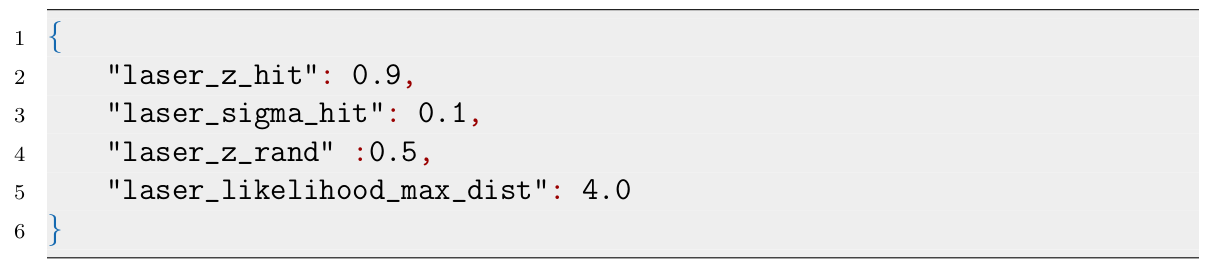
\includegraphics[keepaspectratio, scale=0.3]
      {images/senkou_1.png}
 \caption{Laser-related parameters}
 \label{Fig:laser-related parameters}
\end{figure}

\begin{figure}[hbtp]
  \centering
 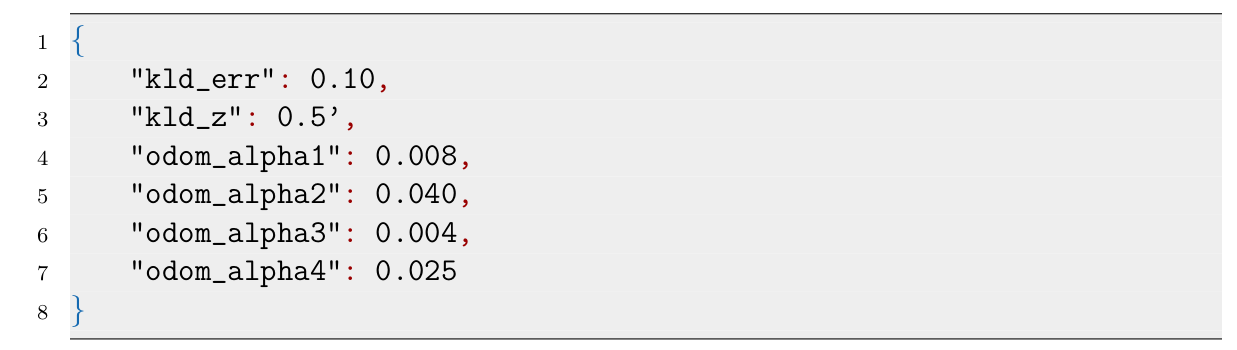
\includegraphics[keepaspectratio, scale=0.3]
      {images/senkou_2.png}
 \caption{Odometry and particle filter parameters}
 \label{Fig:odometry and particle filter parameters}
\end{figure}


\subsection{A guide to implement ROS Navigation Stack on any robot}
ROSのナビゲーションのパラメータ調整について解説されている資料として, A guide to implement ROS Navigation Stack on any robot\cite{siryo_3}が挙げられる. 
このガイドでは, ROS Navigation Stackの主要な構成要素や一部のパラメータ例が紹介されており, シミュレータ上でのナビゲーション実装手順についても解説されている. 

しかし, \figref{Fig:param_example_1}, \figref{Fig:param_example_2}, \figref{Fig:param_example_3}のように具体的な調整方法については明確に示されていない. 
読み手はパラメータの設定値の一例は得られるものの,実際にナビゲーションシステムを向上させるための具体的な調整手順を導き出すことは難しいという課題がある.
\begin{figure}[hbtp]
  \centering
 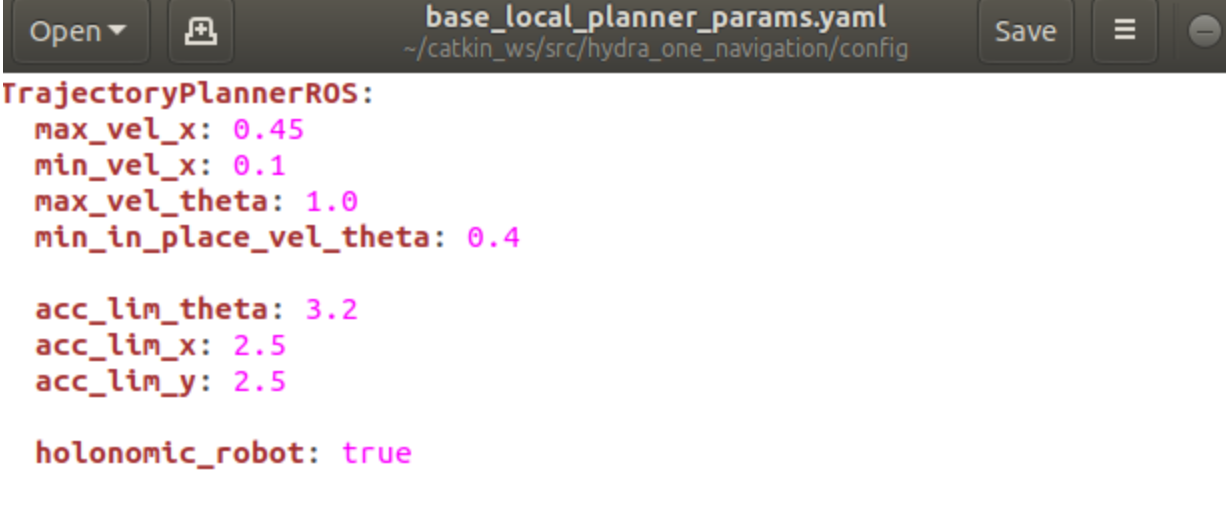
\includegraphics[keepaspectratio, scale=0.17]
      {images/param_example_1.png}
 \caption{Parameters for TrajectoryPlannerROS}
 \label{Fig:param_example_1}
\end{figure}

\begin{figure}[hbtp]
  \centering
 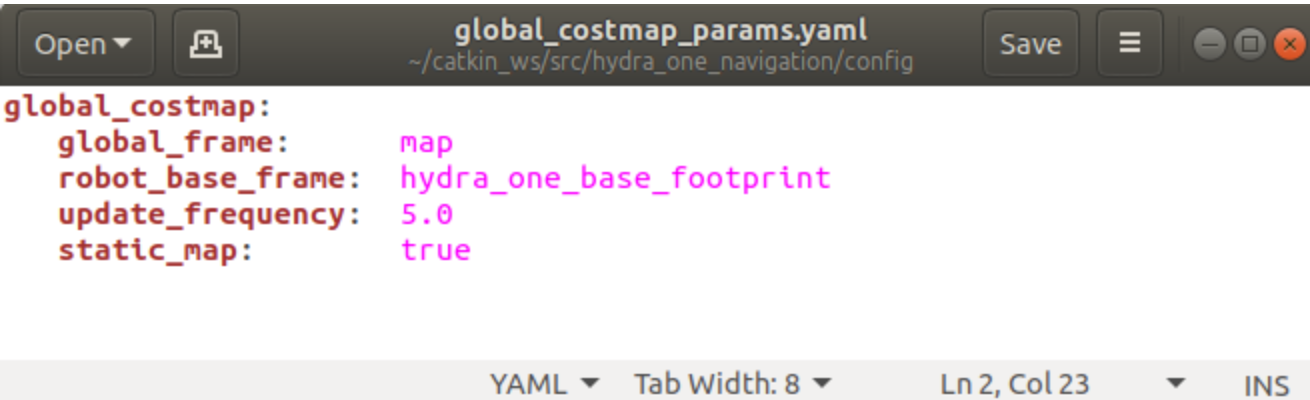
\includegraphics[keepaspectratio, scale=0.17]
      {images/param_example_2.png}
 \caption{Parameters for global costmap}
 \label{Fig:param_example_2}
\end{figure}

\begin{figure}[hbtp]
  \centering
 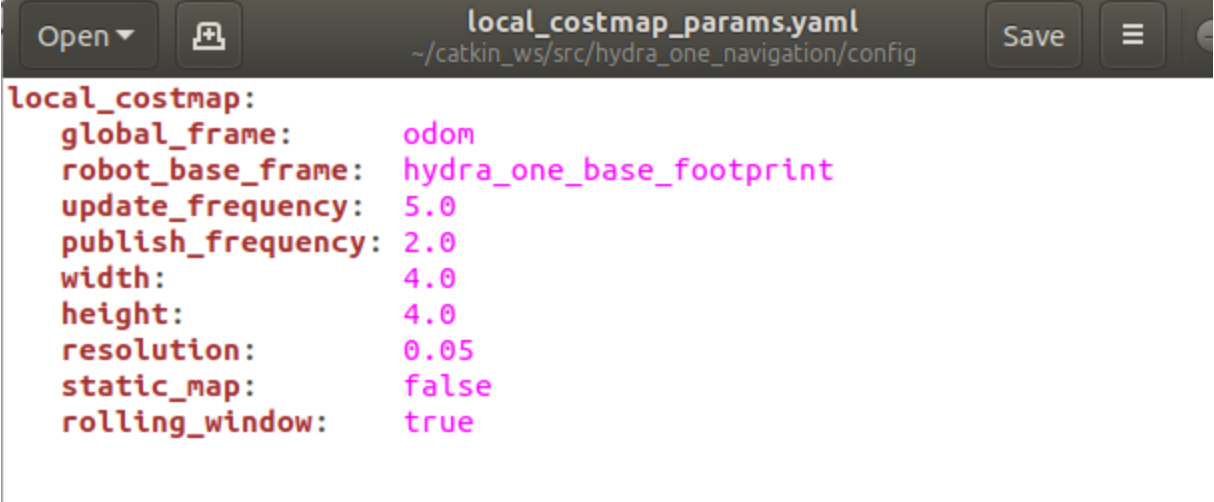
\includegraphics[keepaspectratio, scale=0.17]
      {images/param_example_3.png}
 \caption{Parameter for local costmap}
 \label{Fig:param_example_3}
\end{figure}

\newpage
\section{目的}
本論文では, ロボットにおけるナビゲーションの調整手順を体系化し, 調整方法の一例を示すことを目的とする. 

\section{論文の構成}
本論文では以下のように構成される. 

2章で本研究で使用される要素技術について述べる. 

3章では本研究で作成したドキュメントについて述べる. 

4章では津田沼チャレンジによる実験でドキュメントの有効性を検証する. 

5章ではつくばチャレンジによる実験でドキュメントの有効性を検証する. 

6章では本論文について結論を述べる. 

\newpage

% 2
\chapter{要素技術}
\section{ROS}
ROS(Robot Operating System)は, ロボット開発を効率化するためのオープンソースソフトウェアフレームワークである. 
複数のプログラミング言語向けのライブラリや, センサや状態を可視化するツール群, ノード間のメッセージ通信機構, およびパッケージによるモジュール管理機能を備えている点が特徴である. 
ROSにおける基本的な実行単位はノードであり, ノードはトピックやサービスといった仕組みを通じて情報を交換する. 
これにより, センサデータの取得や制御アルゴリズム, 経路計画などを個別のモジュールとして構成し, 分散して動作させることが可能となる. 
さらに, 既成のアルゴリズムやデバイス向けソフトウェアをパッケージとして利用することで, 開発者は低コストかつ短期間で複雑な機能を実装することができる. 



\section{ナビゲーション}
ROS Navigation stack\cite{navstack}は, 自律移動ロボットが環境内を自律的に移動するためのソフトウェアフレームワークである. 主に以下の要素から構成されている. 
\begin{itemize}
     \item \textbf{自己位置推定}\\
     ロボットは地図上で自己位置を推定する必要がある. その代表的な手法として, AMCL(Adaptive Monte Carlo Localization)が用いられる. 
     AMCLはROS Navigation Stackで自己位置推定を行う確率的アルゴリズムであり, LiDARやオドメトリ情報をもとに多数の仮説(パーティクル)を生成し, 
     それぞれの重みを更新することでロボットの位置を推定する. また, 状況に応じてパーティクル数を動的に調整することで精度と計算負荷のバランスを取る特徴をもつ. 
     一方で, その性能はオドメトリ誤差やレーザノイズなど多くのパラメータ設定に依存しており, 実環境に応じたチューニングが重要となる. 
     \item \textbf{地図生成}\\
     未知領域においては, 環境のマッピングのため, SLAM(Simultaneous Localization and Mapping)が必要となる. 
     SLAMは, ロボットが未知の環境内で自己位置を推定しながら同時に地図を生成するための手法であり, 
     自律移動の基盤技術の一つである. ロボットはLiDARやカメラなどのセンサ情報を取得し, 環境内の特徴点や障害物を検出することで地図を構築すると同時に, 
     自身の位置をその地図上で推定する. この相互依存的な推定を繰り返すことで, 外部基準を持たない環境でも自己位置と地図を同時に確立できる. 
     \item \textbf{経路計画}\\
     経路計画は, ロボットが目的地へ到達するための経路を生成, 追従するプロセスであり, ナビゲーションシステムの中心的な役割を担う. 
     大域的経路計画は, 静的な地図情報をもとに, ロボットの現在位置から目的地までの全体的な経路を計算する段階である. 
     ここでは主にDijkstra法やA*アルゴリズムといったグラフ探索手法が用いられ, 障害物を避けつつコストマップ上で最短または最適な経路を算出する. 
     一方, 局所的経路計画は, ロボットが実際に移動する際の動作をリアルタイムに制御する段階であり, 
     センサ情報をもとに動的な障害物を回避しながら経路を追従する. 
     代表的な手法であるDWA(Dynamic Window Approach)は, ロボットの運動学的制約を考慮しつつ, 
     速度空間内で安全かつ効率的な制御コマンドを探索するアルゴリズムである. 
     DWAは目標方向の進行性, 障害物との距離, 安全性など複数の評価関数を組み合わせて最適な行動を選択することで, 
     滑らかな走行と衝突回避を両立させている. 
     \item \textbf{コストマップ}\\
     コストマップは, ロボットの経路計画において基盤となる情報構造であり, 環境内の障害物や走行困難な領域を数値化して表現することで, 
     経路計画アルゴリズムが安全かつ効率的に移動できるようにする. 
     ROS Navigation stackでは, コストマップは, 静的マップと動的マップにに分けて管理される. 
     静的マップはあらかじめ生成された地図に基づく固定的な障害物情報を提供し, 
     局所的な経路計画や障害物回避の基盤として利用される. 
     一方, 動的マップはLiDARやカメラなどのセンサ情報をもとにリアルタイムで更新され, 
     移動中に出現する人などの動的障害物を反映する. コストマップ上では, 
     障害物が存在するセルの値が高く, 通行可能な領域は低い値で表現される. 
     この数値は経路計画アルゴリズムによって考慮され, ロボットはより安全でコストの低い経路を優先して移動する. 
     これにより, 経路計画は単に障害物を避けるだけでなく, 走行中の安全性を確保しつつ目標地点まで到達できるようになる. 
\end{itemize}
% 3
\chapter{作成したドキュメント}
\section{ドキュメントの構成}
作成したドキュメントの構成は以下の要素から構成されている. 
また, 作成にあたってROS WikiのNavigationページを参考にした.
\cite{ros_wiki_navigation}
\begin{itemize}
     \item \textbf{自己位置推定(AMCL)}
     \begin{itemize}
        \item \textbf{最低限の設定}
        \item \textbf{主要パラメータの調整}
        \item \textbf{その他パラメータの調整}
        \item \textbf{ROS\_ERRORが出たときの問題と対処法}
    \end{itemize}
     \item \textbf{経路計画(Move Base)}
    \begin{itemize}
        \item \textbf{最低限の設定}
        \item \textbf{Move Baseの土台となるパラメータ調整}
        \item \textbf{リカバリ動作のパラメータ調整}
        \item \textbf{コストマップのパラメータ調整}
        \item \textbf{ローカルプランナーのパラメータ調整}
        \item \textbf{グローバルプランナーのパラメータ調整}
        \item \textbf{ROS\_WARNが出たときの問題と対処法}
    \end{itemize}
\newpage
     \item \textbf{地図}
    \begin{itemize}
        \item \textbf{地図作成方法の説明}
        \item \textbf{slam\_toolboxでの地図作成方法}
        \item \textbf{glimでの地図作成方法}
    \end{itemize}
    \item \textbf{オドメトリ}
    \begin{itemize}
        \item \textbf{オドメトリの調整手順}
    \end{itemize}     
\end{itemize}

\section{ドキュメントの例示}
本論文では, 作成したドキュメントの中から例示として, オドメトリ調整と自己位置推定(AMCL)の
2項目を取り上げ, 記載内容の一部を示す. 

\subsection{オドメトリ調整}
調整対象のパラメータは, 車輪半径に関する補正係数であるwheel\_radius\_multiplierと, 車輪環距離に関する補正係数であるwheel\_separation\_multiplierの2つである. 
これらはロボットのオドメトリの正確さに直結するため, 自己位置推定を行う上で最初に調整すべき項目である. 




% 4
\chapter{津田沼チャレンジによるドキュメントの有効性の検証実験}
\section{実験概要}
本研究で作成したドキュメントの有効性を確認するため, 津田沼チャレンジのコースを用いて自律移動実験を行った. 
実験では, ロボットが自律的にナビゲーションを実行し, 設定されたコースを完走できるかを確認することを目的とした. 

実験は, 作成者が2025年度版コースを対象に実施したものと, 学部3年生が2024年度版コースでドキュメントを参照して実施したものの2種類である. 
それぞれのコースを\figref{Fig:Course map of the Tsudanuma Challenge 2025}, \figref{Fig:Course map of the Tsudanuma Challenge 2024}に示す.
作成者の実験では, 走行地図の作成から自己位置推定および経路計画に関する各種パラメータの調整までを一貫して行った. 
一方, 学部3年生による実験では, 作成者がまとめたドキュメントを基に, 作成者が作成した地図を使用してナビゲーションの構築と調整を行った. 

実験に用いたロボットは本研究室で開発されているロボットORNE-box2\cite{井口颯人2023屋外自律移動ロボットプラットフォーム-orne}を使用した. 
その外観を\figref{Fig:ORNE-box2}に示す. 
また, ナビゲーションにはROS Navigation Stackを用いた. 
\begin{figure}[hbtp]
  \centering
 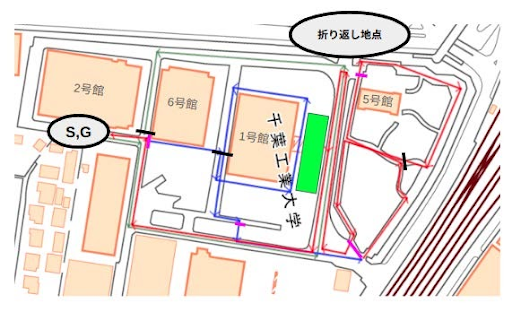
\includegraphics[keepaspectratio, scale=0.5]
      {images/2025tsudacha.png}
 \caption{Course map of the Tsudanuma Challenge 2025(souce: \cite{tsudachare})}
 \label{Fig:Course map of the Tsudanuma Challenge 2025}
\end{figure}
\begin{figure}[hbtp]
  \centering
 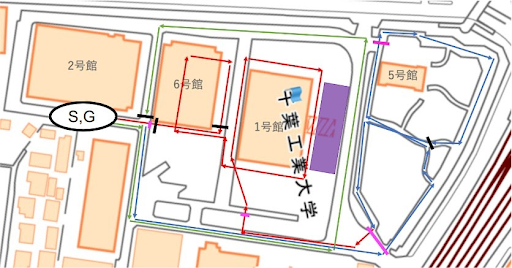
\includegraphics[keepaspectratio, scale=0.5]
      {images/2024tsudacha.png}
 \caption{Course map of the Tsudanuma Challenge 2024(souce: \cite{tsudachare})}
 \label{Fig:Course map of the Tsudanuma Challenge 2024}
\end{figure}
\begin{figure}[hbtp]
  \centering
 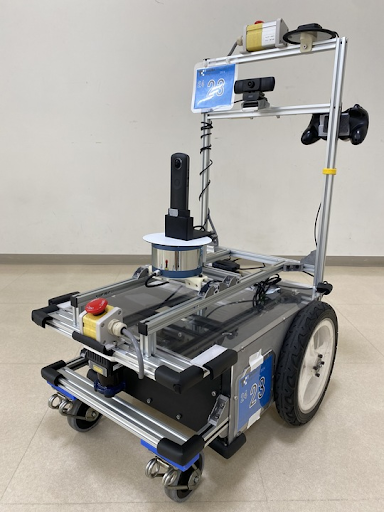
\includegraphics[keepaspectratio, scale=0.3]
      {images/box2.png}
 \caption{ORNE-box2}
 \label{Fig:ORNE-box2}
\end{figure}





\section{実験結果}


\subsection{作成者による結果}


\subsection{学部3年生による結果}
% 5
\chapter{つくばチャレンジによるドキュメントの有効性の検証実験}
\section{実験概要}
本研究で作成したドキュメントの有効性を確認するため, つくばチャレンジ2025\cite{つくばチャレンジ}のコースを用いて自律移動実験を行った. 
実験では, ドキュメントによる手順通りにナビゲーションのパラメータを調整されたロボットが, 自律的に設定されたコースを完走できるかで, ドキュメントの妥当性を確認することを目的とした. 
そのコースを\figref{Fig:Course map of the Tsukuba Challenge 2025}に示す.
実験では, 作成者が走行地図の作成から自己位置推定および経路計画に関する各種パラメータの調整までを全て行った. 

実験には, 本研究室で開発されているロボットORNE-box2を使用した. 
また, ナビゲーションにはROS Navigation stackを用いた. 
\begin{figure}[hbtp]
  \centering
 \includegraphics[keepaspectratio, scale=0.3]
      {images/course_2025.png}
 \caption{Course map of the Tsukuba Challenge 2025(souce: \cite{つくばチャレンジ})}
 \label{Fig:Course map of the Tsukuba Challenge 2025}
\end{figure}

\newpage
\section{実験結果}
% 表
\tabref{}に示すように, 
% 6
\chapter{結論}
本研究では, ROSベースの自律移動ロボットのナビゲーションにおけるパラメータ調整手順を整理したドキュメントを作成し, その有効性を検証した. 
ドキュメントはROS Navigation stackのパラメータを中心に構成されている. 
津田沼チャレンジの実験では, 作成者自身および利用者のいずれもがそのコースを完走し, ドキュメントが有効であることを確認した. 
また, つくばチャレンジ2025において, 
%ここにディレクトリのパスを追加していく
%
%% Back Matter
\backmatter{}
%
\section{ROS}
ROS(Robot Operating System)は, ロボット開発を効率化するためのオープンソースソフトウェアフレームワークである. 
複数のプログラミング言語向けのライブラリや, センサや状態を可視化するツール群, ノード間のメッセージ通信機構, およびパッケージによるモジュール管理機能を備えている点が特徴である. 
ROSにおける基本的な実行単位はノードであり, ノードはトピックやサービスといった仕組みを通じて情報を交換する. 
これにより, センサデータの取得や制御アルゴリズム, 経路計画などを個別のモジュールとして構成し, 分散して動作させることが可能となる. 
さらに, 既成のアルゴリズムやデバイス向けソフトウェアをパッケージとして利用することで, 開発者は低コストかつ短期間で複雑な機能を実装することができる. 



\section{ナビゲーション}
ROS Navigation stack\cite{navstack}は, 自律移動ロボットが環境内を自律的に移動するためのソフトウェアフレームワークである. 主に以下の要素から構成されている. 
\begin{itemize}
     \item \textbf{自己位置推定}\\
     ロボットは地図上で自己位置を推定する必要がある. その代表的な手法として, AMCL(Adaptive Monte Carlo Localization)が用いられる. 
     AMCLはROS Navigation Stackで自己位置推定を行う確率的アルゴリズムであり, LiDARやオドメトリ情報をもとに多数の仮説(パーティクル)を生成し, 
     それぞれの重みを更新することでロボットの位置を推定する. また, 状況に応じてパーティクル数を動的に調整することで精度と計算負荷のバランスを取る特徴をもつ. 
     一方で, その性能はオドメトリ誤差やレーザノイズなど多くのパラメータ設定に依存しており, 実環境に応じたチューニングが重要となる. 
     \item \textbf{地図生成}\\
     未知領域においては, 環境のマッピングのため, SLAM(Simultaneous Localization and Mapping)が必要となる. 
     SLAMは, ロボットが未知の環境内で自己位置を推定しながら同時に地図を生成するための手法であり, 
     自律移動の基盤技術の一つである. ロボットはLiDARやカメラなどのセンサ情報を取得し, 環境内の特徴点や障害物を検出することで地図を構築すると同時に, 
     自身の位置をその地図上で推定する. この相互依存的な推定を繰り返すことで, 外部基準を持たない環境でも自己位置と地図を同時に確立できる. 
     \item \textbf{経路計画}\\
     経路計画は, ロボットが目的地へ到達するための経路を生成, 追従するプロセスであり, ナビゲーションシステムの中心的な役割を担う. 
     大域的経路計画は, 静的な地図情報をもとに, ロボットの現在位置から目的地までの全体的な経路を計算する段階である. 
     ここでは主にDijkstra法やA*アルゴリズムといったグラフ探索手法が用いられ, 障害物を避けつつコストマップ上で最短または最適な経路を算出する. 
     一方, 局所的経路計画は, ロボットが実際に移動する際の動作をリアルタイムに制御する段階であり, 
     センサ情報をもとに動的な障害物を回避しながら経路を追従する. 
     代表的な手法であるDWA(Dynamic Window Approach)は, ロボットの運動学的制約を考慮しつつ, 
     速度空間内で安全かつ効率的な制御コマンドを探索するアルゴリズムである. 
     DWAは目標方向の進行性, 障害物との距離, 安全性など複数の評価関数を組み合わせて最適な行動を選択することで, 
     滑らかな走行と衝突回避を両立させている. 
     \item \textbf{コストマップ}\\
     コストマップは, ロボットの経路計画において基盤となる情報構造であり, 環境内の障害物や走行困難な領域を数値化して表現することで, 
     経路計画アルゴリズムが安全かつ効率的に移動できるようにする. 
     ROS Navigation stackでは, コストマップは, 静的マップと動的マップにに分けて管理される. 
     静的マップはあらかじめ生成された地図に基づく固定的な障害物情報を提供し, 
     局所的な経路計画や障害物回避の基盤として利用される. 
     一方, 動的マップはLiDARやカメラなどのセンサ情報をもとにリアルタイムで更新され, 
     移動中に出現する人などの動的障害物を反映する. コストマップ上では, 
     障害物が存在するセルの値が高く, 通行可能な領域は低い値で表現される. 
     この数値は経路計画アルゴリズムによって考慮され, ロボットはより安全でコストの低い経路を優先して移動する. 
     これにより, 経路計画は単に障害物を避けるだけでなく, 走行中の安全性を確保しつつ目標地点まで到達できるようになる. 
\end{itemize}
%

\end{document}
